% =====================================================================
%  Chapitre 6 -- Évaluation, interprétabilité et projet
%  Partie b : interprétabilité, Grad-CAM, robustesse, projet GTSRB
% =====================================================================

\begin{frame}{Interprétabilité : pourquoi ouvrir la boîte noire}
\begin{columns}[t]
\begin{column}{0.48\textwidth}
\begin{itemize}
  \item Un CNN donne une réponse, rarement une \textbf{justification}.
  \item En contexte critique (santé, transport), il faut pouvoir
  \emph{expliquer} la décision.
  \item L'interprétabilité sert aussi à \textbf{déboguer} : un modèle qui regarde
  le fond de l'image au lieu du panneau a « appris » un raccourci.
\end{itemize}
\begin{kbox}[Trois niveaux d'observation]
\begin{enumerate}
  \item Les \textbf{poids} (les filtres eux-mêmes).
  \item Les \textbf{activations} (ce que voit une couche sur une image).
  \item La \textbf{salle} (quelle région a pesé dans la décision) : Grad-CAM.
\end{enumerate}
\end{kbox}
\end{column}
\begin{column}{0.48\textwidth}
\begin{wbox}[Un piège classique]
Un classifieur de « loup » peut ne s'appuyer que sur la \textbf{neige} du fond.
Il a 95 \% d'exactitude\dots{} et il est inutilisable hors hiver.
Seule la visualisation révèle ce genre de biais.
\end{wbox}
\end{column}
\end{columns}
\end{frame}

\begin{frame}{Visualiser les filtres appris}
\begin{columns}[t]
\begin{column}{0.54\textwidth}
\centering
\end{column}
\begin{column}{0.42\textwidth}
\begin{itemize}
  \item Un filtre $3\times3$ est une petite matrice de \textbf{9 poids}.
  \item On peut l'afficher : chaque case est une valeur, du sombre (négatif)
  au clair (positif).
  \item En première couche, ces noyaux ressemblent souvent à des
  \textbf{détecteurs de contours} ou de \textbf{dégradés}.
  \item Ils ne sont pas fixés à la main : ils sont \textbf{appris}.
\end{itemize}
\begin{kbox}[Lecture]
Un noyau qui a un côté clair et un côté sombre réagit à un \textbf{gradient}
de luminosité, donc à un contour.
\end{kbox}
\end{column}
\end{columns}
% [fix] figure sortie
\end{frame}

\begin{frame}{Visualiser les filtres appris --- la figure}\begin{center}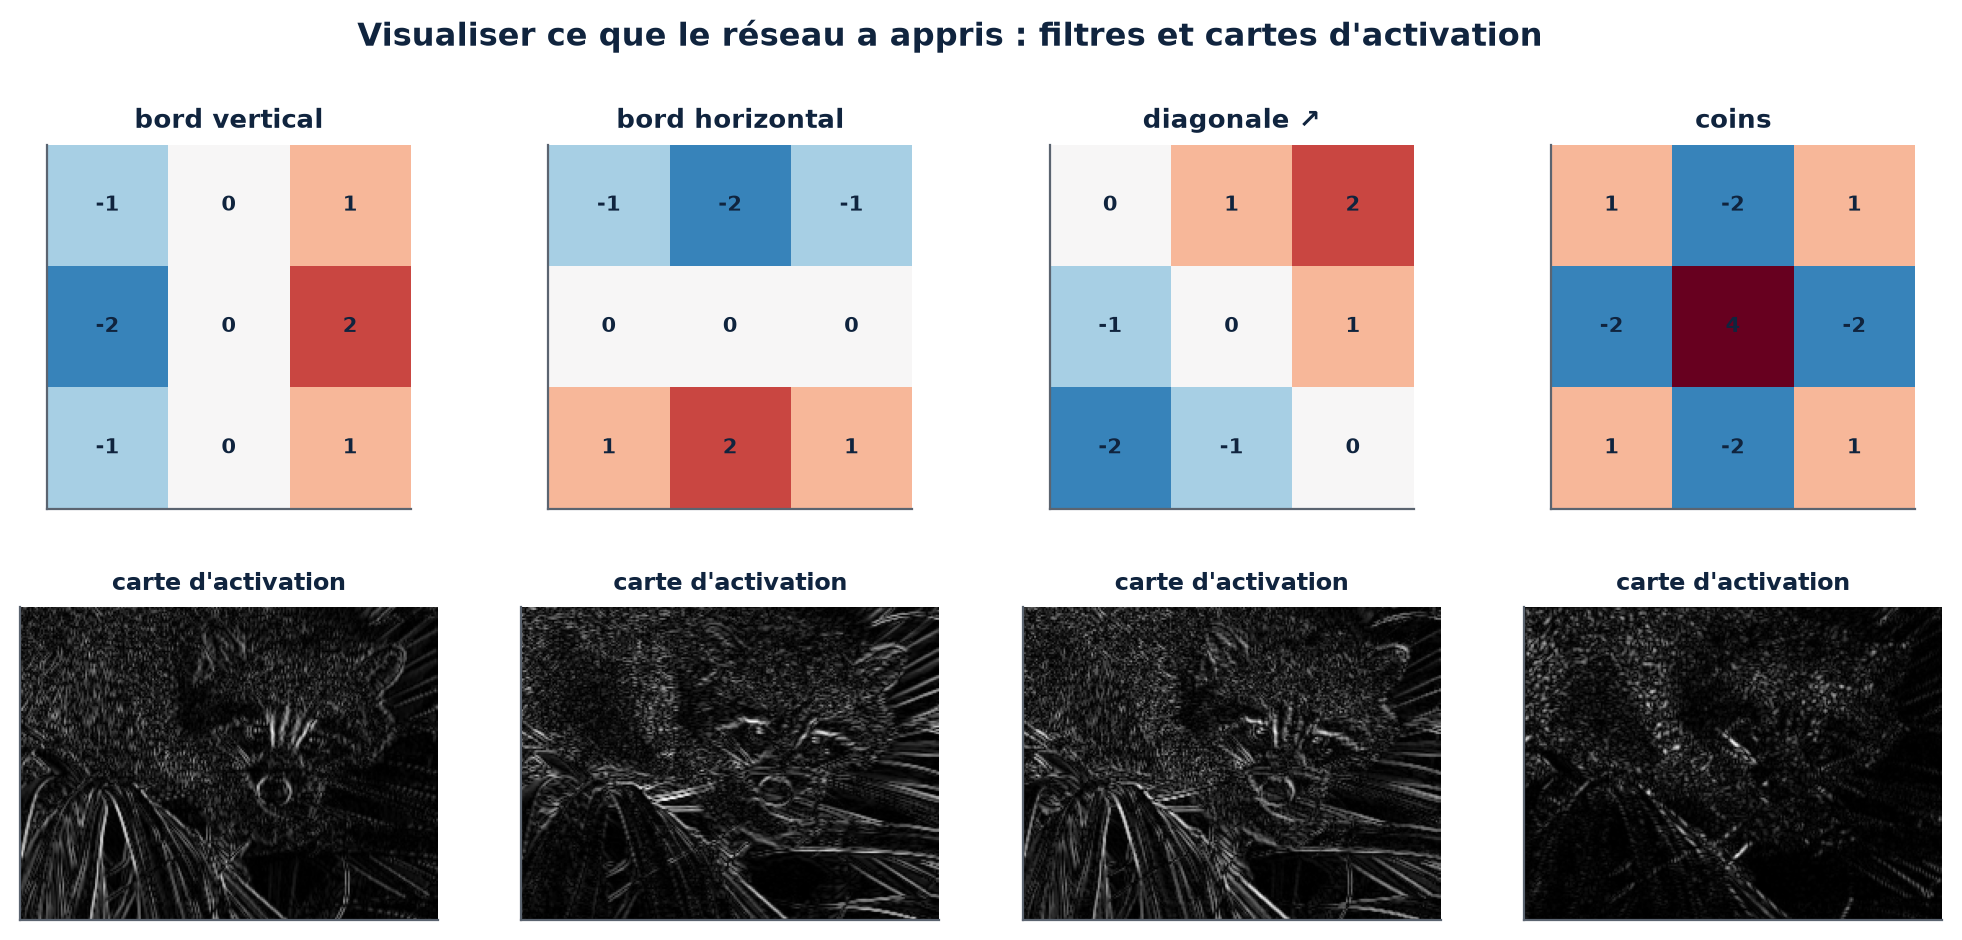
\includegraphics[width=.92\textwidth]{k04_filtres_activations.png}\end{center}\end{frame}

\begin{frame}{Les cartes d'activation}
\begin{columns}[t]
\begin{column}{0.48\textwidth}
\begin{itemize}
  \item On applique un filtre à toute l'image : on obtient une
  \textbf{carte d'activation} (\emph{feature map}).
  \item Les zones où le motif est détecté s'allument.
  \item Une couche produit \textbf{autant de cartes} que de filtres.
  \item Ces cartes sont empilées : c'est le \textbf{tenseur de sortie}
  de la couche.
\end{itemize}
\end{column}
\begin{column}{0.48\textwidth}
\begin{ebox}[Le même noyau, partout]
Un filtre détecte \emph{le même} motif en tout point de l'image : c'est le
partage de poids. La carte d'activation est donc une \textbf{carte de présence}
du motif.
\end{ebox}
\begin{wbox}[Attention]
Une activation forte ne signifie pas « c'est important pour la classe » : elle
signifie seulement « le motif est là ». Grad-CAM répond à l'autre question.
\end{wbox}
\end{column}
\end{columns}
\end{frame}

\begin{frame}{La hiérarchie des caractéristiques}
\begin{center}
\begin{tikzpicture}[node distance=4mm,>=Latex,
  box/.style={draw=byDeep!40,fill=byLight,rounded corners=1.5mm,
              minimum width=3.2cm,minimum height=1.35cm,align=center,font=\scriptsize}]
\node[box] (a) {\textbf{Couche 1}\\[1pt]bords, taches\\de couleur};
\node[box,right=of a] (b) {\textbf{Couches 2--3}\\[1pt]coins, arcs,\\motifs simples};
\node[box,right=of b] (c) {\textbf{Couches 4--5}\\[1pt]parties d'objet\\(roue, vitre)};
\node[box,right=of c] (d) {\textbf{Couches denses}\\[1pt]objet complet\\\emph{voiture}};
\draw[->,thick,byBlue] (a)--(b);
\draw[->,thick,byBlue] (b)--(c);
\draw[->,thick,byBlue] (c)--(d);
\end{tikzpicture}
\end{center}
\vspace{1mm}
\begin{columns}[t]
\begin{column}{0.48\textwidth}
\begin{itemize}
  \item Chaque bloc de convolution élargit le \textbf{champ récepteur}.
  \item En profondeur, un neurone « voit » une région de plus en plus grande.
  \item Le réseau construit donc une \textbf{composition} : bord $\to$ partie
  $\to$ objet.
\end{itemize}
\end{column}
\begin{column}{0.48\textwidth}
\begin{kbox}[Conséquence pratique]
Le \textbf{transfert} fonctionne pour cette raison : les premières couches
apprennent des motifs génériques, réutilisables sur une autre tâche.
\end{kbox}
\end{column}
\end{columns}
\end{frame}

\begin{frame}[fragile]{Grad-CAM : le principe}
\begin{columns}[t]
\begin{column}{0.50\textwidth}
\begin{itemize}
  \item On choisit une \textbf{classe cible} $c$ et une \textbf{couche
  convolutive} (la dernière).
  \item On calcule le gradient du score $y^c$ par rapport à chaque carte $A^k$.
  \item On le moyenne spatialement : cela donne un \textbf{poids} $\alpha_k^c$.
  \item On combine les cartes pondérées, puis on garde le positif.
\end{itemize}
\[ \alpha_k^c = \frac{1}{Z}\sum_{i,j}
   \frac{\partial y^c}{\partial A^k_{ij}}
   \qquad
   L^c = \mathrm{ReLU}\!\Big(\sum_k \alpha_k^c A^k\Big) \]
\end{column}
\begin{column}{0.46\textwidth}
\begin{codebox}[Grad-CAM en quelques lignes]
\begin{lstlisting}
# activations = sortie de la
# derniere couche conv
act = couche_conv.sortie
act.retain_grad()
score = sortie[:, classe]
score.backward()
# poids = moyenne spatiale
#         du gradient
poids = act.grad.mean((2, 3))
cam = (poids[:, :, None, None]
       * act).sum(1)
cam = cam.clamp(min=0)
\end{lstlisting}
\end{codebox}
\end{column}
\end{columns}
\end{frame}

\begin{frame}{Grad-CAM : ce que l'on voit}
\begin{columns}[t]
\begin{column}{0.56\textwidth}
\centering
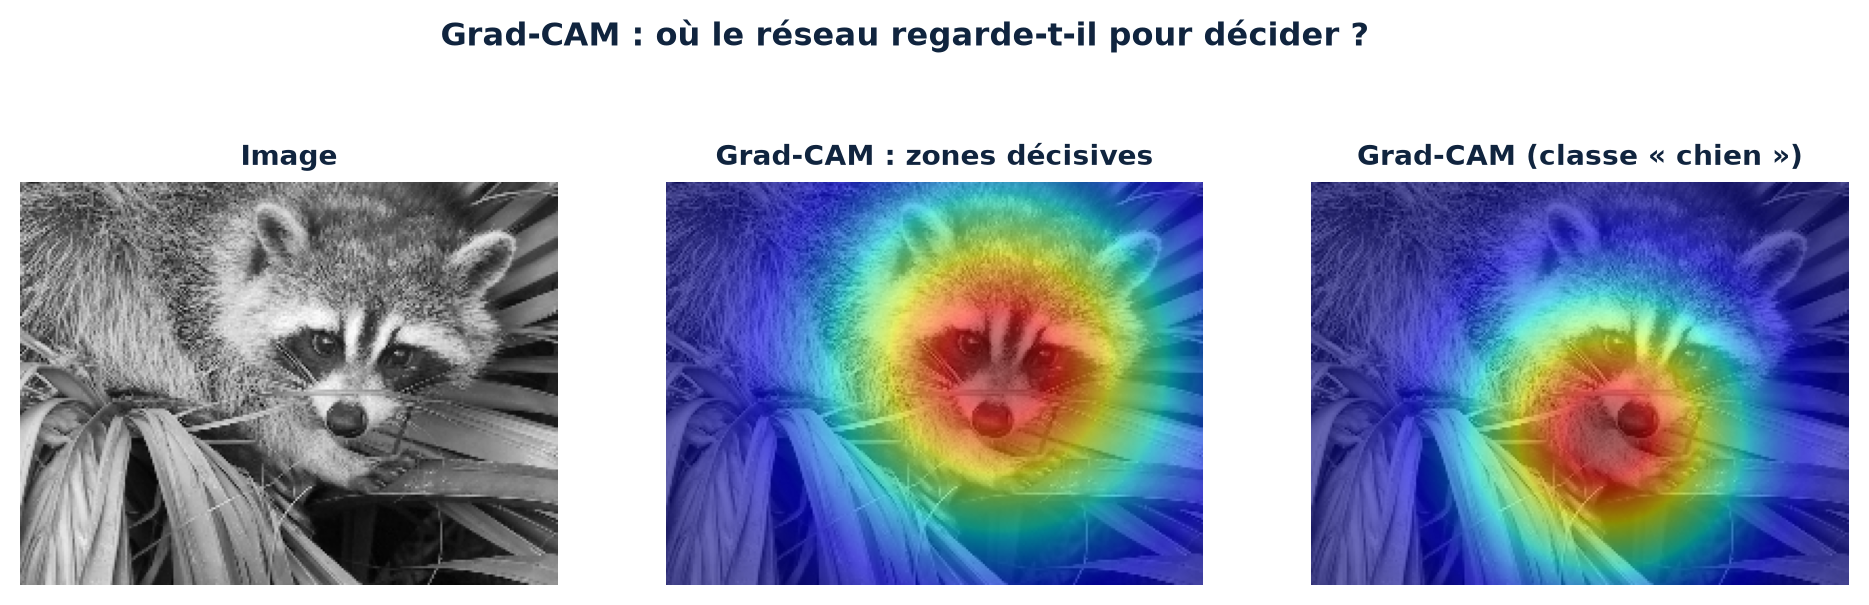
\includegraphics[width=0.54\textwidth]{k05_gradcam.png}
\end{column}
\begin{column}{0.40\textwidth}
\begin{itemize}
  \item La carte $L^c$ est \textbf{surimposée} à l'image d'origine.
  \item Les zones chaudes sont celles qui ont fait \emph{pencher} la décision
  vers la classe $c$.
  \item Sur un panneau, la carte se concentre sur le \textbf{pictogramme},
  pas sur le ciel ni la route.
\end{itemize}
\begin{kbox}[Le test de confiance]
Si la carte s'allume \emph{hors} de l'objet, le modèle s'appuie sur un
\textbf{artefact} : il est fragile.
\end{kbox}
\end{column}
\end{columns}
\end{frame}

\begin{frame}{Robustesse : la chute sous perturbation}
\begin{columns}[t]
\begin{column}{0.54\textwidth}
\centering
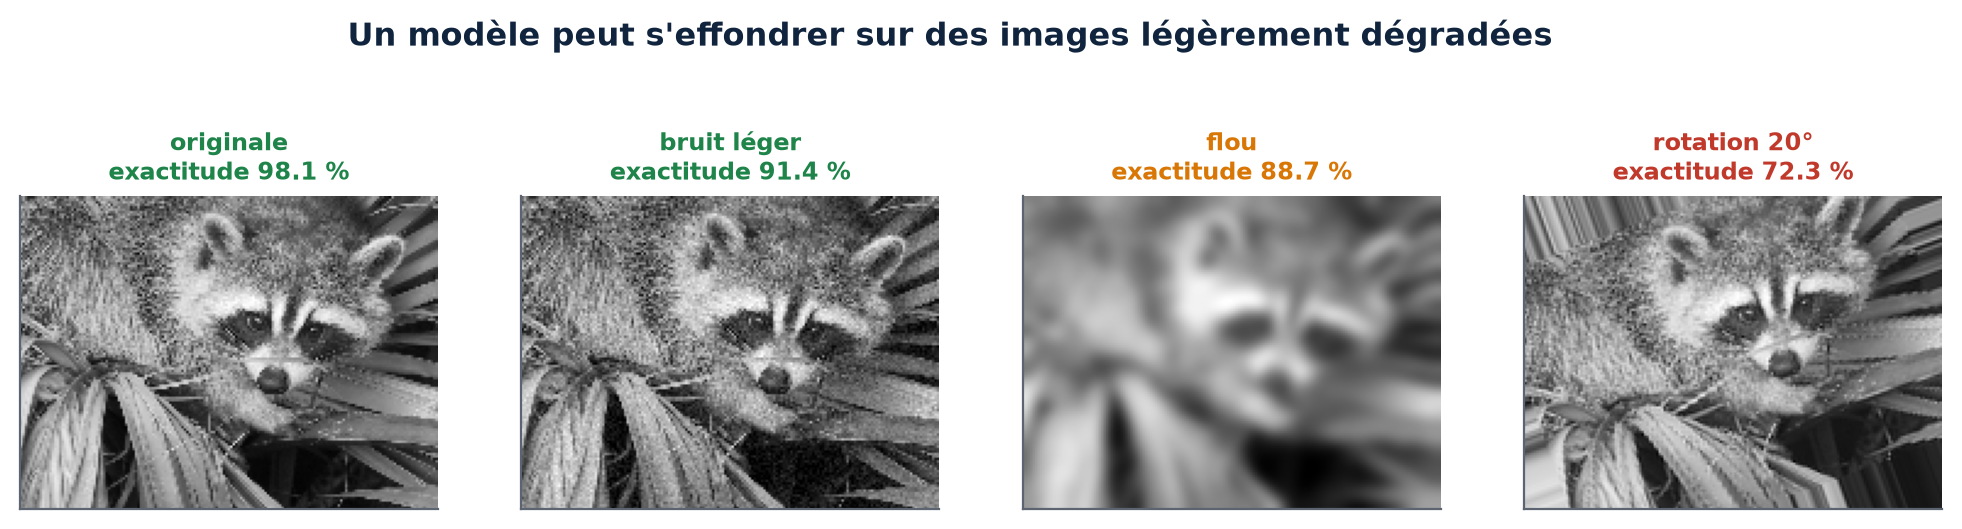
\includegraphics[width=0.52\textwidth]{k06_robustesse.png}
\end{column}
\begin{column}{0.42\textwidth}
\begin{center}
\footnotesize
\begin{tabular}{@{}lr@{}}
\toprule
\textbf{Condition} & \textbf{Exactitude} \\
\midrule
Image originale      & 98,1 \% \\
Bruit léger          & 91,4 \% \\
Flou                 & 88,7 \% \\
Rotation $20^\circ$  & \textbf{72,3 \%} \\
\bottomrule
\end{tabular}
\end{center}
\begin{wbox}[26 points perdus]
Une simple rotation de $20^\circ$ fait tomber l'exactitude de \textbf{98,1 \%}
à \textbf{72,3 \%}. Le réseau n'a pas appris l'invariance qu'on lui prêtait.
\end{wbox}
\end{column}
\end{columns}
\end{frame}

\begin{frame}{Exemples adversariaux et biais de données}
\begin{columns}[t]
\begin{column}{0.48\textwidth}
\begin{wbox}[Exemples adversariaux]
On ajoute à l'image un bruit \emph{imperceptible à l'œil} mais calculé pour
tromper le réseau. La classe change, l'image semble identique.
\begin{itemize}
  \item Révèle que la décision repose sur des détails fragiles.
  \item Se transfère d'un modèle à l'autre.
\end{itemize}
\end{wbox}
\end{column}
\begin{column}{0.48\textwidth}
\begin{kbox}[Biais de jeu de données]
Le modèle hérite des défauts des données :
\begin{itemize}
  \item classes sous-représentées ;
  \item conditions absentes (nuit, pluie, neige) ;
  \item annotations incohérentes.
\end{itemize}
Un jeu « propre » donne un modèle « propre » --- et aveugle ailleurs.
\end{kbox}
\end{column}
\end{columns}
\vspace{1mm}
\begin{ebox}[La réponse pratique]
Augmentation ciblée (rotations, changements de luminosité), jeux plus variés,
et \textbf{évaluation par sous-groupe} plutôt qu'une moyenne globale.
\end{ebox}
\end{frame}

\begin{frame}{Le projet : classifier les panneaux GTSRB}
\begin{columns}[t]
\begin{column}{0.52\textwidth}
\begin{abox}[Le cahier des charges]
\begin{itemize}
  \item Entrées : 39\,209 images d'entraînement, 12\,630 de test, 43 classes.
  \item Sortie : une classe parmi 43, avec top-3.
  \item Contrainte : entraînement sur \textbf{CPU}, en temps raisonnable.
  \item Livrable : un rapport court avec métriques et matrice de confusion.
\end{itemize}
\end{abox}
\end{column}
\begin{column}{0.44\textwidth}
\begin{kbox}[Les étapes]
\begin{enumerate}
  \item Explorer et redimensionner ($32\times32$).
  \item Découper train / validation / test.
  \item Construire un petit CNN.
  \item Entraîner, lire les courbes.
  \item Augmenter les données, comparer.
  \item Évaluer : matrice, $P$, $R$, $F1$, top-3.
  \item Visualiser avec Grad-CAM.
\end{enumerate}
\end{kbox}
\end{column}
\end{columns}
\end{frame}

\begin{frame}{Projet : ce qui est attendu, ce qui est sanctionné}
\begin{columns}[t]
\begin{column}{0.48\textwidth}
\begin{ebox}[Ce qui est valorisé]
\begin{itemize}
  \item Un découpage \textbf{propre} et justifié.
  \item Une comparaison \emph{chiffrée} de deux configurations.
  \item Un diagnostic des classes confondues.
  \item Une figure Grad-CAM commentée.
\end{itemize}
\end{ebox}
\end{column}
\begin{column}{0.48\textwidth}
\begin{wbox}[Ce qui coûte des points]
\begin{itemize}
  \item Régler les hyperparamètres sur le jeu de \textbf{test}.
  \item Annoncer une exactitude sans matrice ni $F1$.
  \item Un « ça marche » sans courbe ni analyse d'erreurs.
  \item Des chiffres non reproductibles (pas de graine fixée).
\end{itemize}
\end{wbox}
\end{column}
\end{columns}
\vspace{1mm}
\begin{kbox}[Repères de performance]
CNN simple $\approx$ 88,2 \% (top-1) ; avec augmentation 94,6 \% ;
transfert VGG-16 98,1 \%. Atteindre l'ordre de 90 \% sur CPU est un bon résultat.
\end{kbox}
\end{frame}

\begin{frame}{Quiz de fin de chapitre}
\begin{qbox}[Question 1]
Un modèle annonce 95 \% d'exactitude sur un jeu où une classe représente
1 \% des images. Que faut-il vérifier en priorité ?
\begin{itemize}
  \item[(a)] Le temps d'entraînement \quad (b) Le rappel et le $F1$ de cette classe
  \quad (c) La taille du modèle
\end{itemize}
\end{qbox}
\begin{qbox}[Question 2]
Dans une matrice de confusion, que représente un élément hors diagonale ?
\begin{itemize}
  \item[(a)] Une image mal labellisée \quad (b) Une confusion entre la classe réelle
  (ligne) et la classe prédite (colonne) \quad (c) Un paramètre du réseau
\end{itemize}
\end{qbox}
\begin{qbox}[Question 3]
Que mesure le top-3 ?
\begin{itemize}
  \item[(a)] La précision sur trois images \quad (b) La proportion de cas où la bonne
  classe figure parmi les trois meilleures propositions \quad (c) Trois époques
\end{itemize}
\end{qbox}

% [fix] bloc deplace
% [fix] bloc deplace
\end{frame}
\begin{frame}{Quiz de fin de chapitre (suite)}
\begin{qbox}[Question 4]
Grad-CAM s'appuie sur\dots

\end{qbox}
\end{frame}
\begin{frame}{Quiz de fin de chapitre (suite)}
\begin{itemize}
  \item[(a)] les poids de la première couche \quad (b) le gradient de la classe cible
  par rapport à la dernière carte convolutive \quad (c) la matrice de confusion
\end{itemize}
\end{frame}

\begin{frame}{Réponses du quiz}
\begin{solbox}[Réponses --- à ne regarder qu'après avoir répondu]
\textbf{1.} (b) : sur des classes déséquilibrées, l'exactitude noie la classe rare ;
il faut regarder son rappel et son $F1$. \quad
\textbf{2.} (b) : la ligne est la vérité, la colonne la prédiction ; hors diagonale,
le modèle s'est trompé de classe. \quad
\textbf{3.} (b) : on tolère trois propositions ; utile quand les erreurs proches sont
acceptables. \quad
\textbf{4.} (b) : les gradients moyennés donnent le poids de chaque carte, puis on
combine et on garde le positif.
\end{solbox}
\vspace{1mm}
\begin{wbox}[Le fil rouge]
Toutes ces questions portent sur la même idée : \textbf{ne jamais juger un modèle
sur un seul nombre}. Il faut une métrique adaptée, un diagnostic des erreurs et
un regard sur ce qu'il regarde.
\end{wbox}
\end{frame}

\begin{frame}{À retenir --- le chapitre en une page}
\begin{columns}[t]
\begin{column}{0.48\textwidth}
\begin{kbox}[Évaluer]
\begin{itemize}
  \item Trois jeux : MNIST, CIFAR-10, \textbf{GTSRB} (43 classes).
  \item Découpage train / val / test, sans fuite.
  \item Exactitude, précision, rappel, $F1$, matrice de confusion.
  \item Top-$k$ et ROC / AUC pour nuancer.
  \item L'exactitude seule est trompeuse.
\end{itemize}
\end{kbox}
\end{column}
\begin{column}{0.48\textwidth}
\begin{kbox}[Comprendre et douter]
\begin{itemize}
  \item Filtres = noyaux appris ; activations = présence du motif.
  \item Hiérarchie bord $\to$ partie $\to$ objet.
  \item \textbf{Grad-CAM} : où le modèle regarde.
  \item Robustesse : 98,1 \% $\to$ 72,3 \% sous rotation.
  \item Adversarial et biais : les limites réelles.
\end{itemize}
\end{kbox}
\end{column}
\end{columns}
\vspace{1mm}
\begin{ebox}[La phrase à retenir]
Un bon modèle n'est pas celui qui a la meilleure exactitude : c'est celui dont on
sait \textbf{pourquoi} il se trompe, et \textbf{où} il regarde.
\end{ebox}
\end{frame}

\begin{frame}{Passons au projet}
\begin{columns}[t]
\begin{column}{0.58\textwidth}
\begin{abox}[Notebook du projet]
\file{notebooks/PROJET\_GTSRB\_panneaux.ipynb}
\medskip

Il contient, dans l'ordre :
\begin{enumerate}
  \item le chargement et l'exploration de GTSRB ;
  \item le redimensionnement et le découpage ;
  \item un CNN de référence et son entraînement ;
  \item l'évaluation (matrice, $F1$, top-3) ;
  \item une visualisation Grad-CAM à commenter.
\end{enumerate}
\end{abox}
\end{column}
\begin{column}{0.38\textwidth}
\begin{kbox}[À faire pour la séance]
\begin{itemize}
  \item Ouvrir le notebook et exécuter la première cellule.
  \item Vérifier que GTSRB est bien présent en local.
  \item Noter le temps d'une époque sur votre machine.
\end{itemize}
\end{kbox}
\end{column}
\end{columns}
\vspace{1mm}
\begin{wbox}[Rappel]
Tout tourne sur \textbf{CPU} : sous-ensemble de données, peu d'époques, petit
modèle. Un résultat honnête et analysé vaut mieux qu'un chiffre gonflé.
\end{wbox}
\end{frame}
